\documentclass[12pt]{article}

% Language setting
% Replace `english' with e.g. `spanish' to change the document language
\usepackage[english]{babel}

% Set page size and margins
% Replace `letterpaper' with`a4paper' for UK/EU standard size
\usepackage[letterpaper,top=2cm,bottom=2cm,left=3cm,right=3cm,marginparwidth=1.75cm]{geometry}



% Useful packages
\usepackage{amsmath}
\usepackage{graphicx}
\usepackage{float}
\usepackage{indentfirst}
\usepackage{changepage}
\usepackage[colorlinks=true, allcolors=blue]{hyperref}

\setlength{\parindent}{0pt}
\begin{document}


\begin{titlepage}
    \centering

    \vspace*{5cm}

    {\Large ELEN20006\_ 2026\_ SM1 \par}
    {\Huge Digital System \par}
    {\Huge Digital Watch Project Report \par}
    \vspace{2cm}

    {\large Author \par}
    \large{\begin{tabular}{c l}
            1550486 & Selina Cheng \\
        \end{tabular}}

    \begin{center}

        \vspace{1cm}

        \textbf{Acknowledgement}

        \vspace{0.3cm}

        The author would like to acknowledge Anita Cheng for her contribution and support during the development of this project.
    \end{center}
    \vspace{6cm}

    {\large University of Melbourne \par}
    {\large \today \par}

\end{titlepage}
%=======================================================================
%PAGE 1
%=======================================================================
\section{Backup Strategy}

This project uses Git for data backup and version control. The forked repository is stored in the personal account on GitHub.
The committed code is pushed to the remote repository after each module is completed and tested. This ensures that the latest version of the code is always backed up and can be easily accessed from any location.

\section{Waveform Graph}

\subsection{Seven-segment Display Decoder for Dexadecimal Digits} //module 6.1 p.17


\begin{figure}[H]
    \centering
    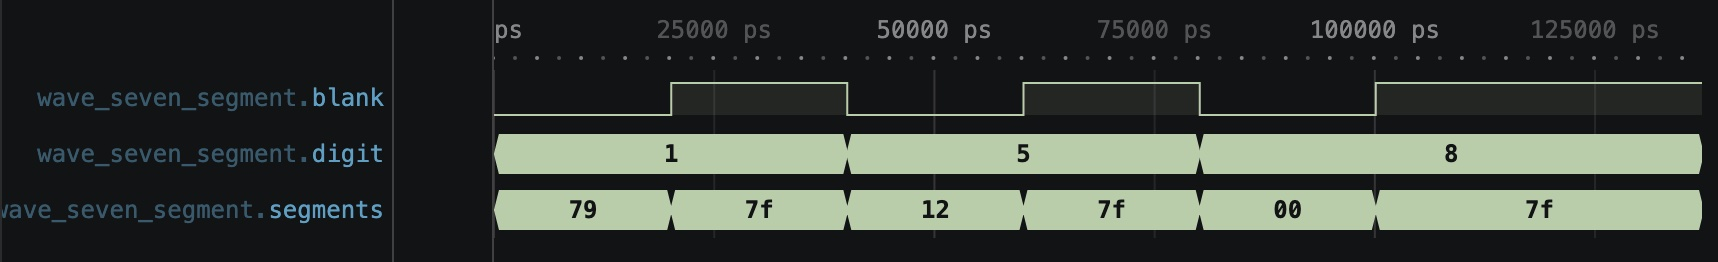
\includegraphics[width=0.9\linewidth]{figures/seven_segment.jpg}
    \caption{Waveform for \texttt{seven\_segment}.}
\end{figure}

\begin{adjustwidth}{2em}{0em}
    Signal values are shown in hexadecimal. When blank is high, the output is 7f, which corresponds to 1111111 in binary — correct for an active-low display. The waveforms confirm the expected behaviour.
\end{adjustwidth}
%Module 6.2 p.18
//module 6.2
\subsection{Parametrised Up-Down Counter with Enable} //module 6.2 p.18

\begin{figure}[H]
    \centering
    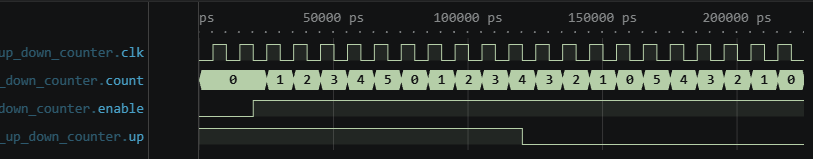
\includegraphics[width=0.9\linewidth]{figures/up_down_counter.png}
    \caption{Waveform for \texttt{up\_down\_counter}.}
\end{figure}

\begin{adjustwidth}{2em}{0em}
    Count values are shown in decimal. When enable is high, the counter starts to count. When up is high, the counter increments by one at every rising edge of the clock and goes down when up is low. The testbech sets MAX to 5, so the counter wraps around to 0 when it reaches 5 and wraps around to 5 when it goes down from 0. The waveforms confirm the expected behaviour.
\end{adjustwidth}
//module 6.3
\subsection{Binary to Binary-Coded Decimal} //module 6.3 p.20

\begin{figure}[H]
    \centering
    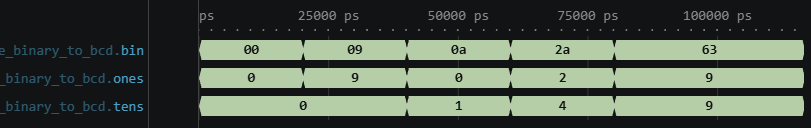
\includegraphics[width=0.9\linewidth]{figures/binary_to_bcd.png}
    \caption{Waveform for \texttt{binary\_to\_bcd}.}
\end{figure}

\begin{adjustwidth}{2em}{0em}
    The binary inputs are shown in hexadecimal. The output values for tens and ones correspond to the tens and ones digits of the binary input in BCD format immediately. For example, when the binary input is 0a, which corresponds to 10 in decimal, tens changes to 1 and ones changes to 0 at the same instance. So,the waveforms confirm the expected behaviour.
\end{adjustwidth}
\subsection{Cascaded Hour-Minute-Second Counter with Enable} //module 6.4 p.20

\begin{figure}[H]
    \centering
    \includegraphics[width=0.9\linewidth]{figures/hms_counter.png}
    \caption{Waveform for \texttt{hms\_counter}.}
\end{figure}

\begin{adjustwidth}{2em}{0em}
    
\end{adjustwidth}
\subsection{Template} //module X.Y p.Z

\begin{figure}[H]
    \centering
    \includegraphics[width=0.9\linewidth]{figures/.png}
    \caption{Waveform for \texttt{}.}
\end{figure}

\begin{adjustwidth}{2em}{0em}
    
\end{adjustwidth}
\subsection{Template} //module X.Y p.Z
\begin{figure}[H]
    \centering
    \includegraphics[width=0.9\linewidth]{figures/.png}
    \caption{Waveform for \texttt{}.}
\end{figure}

\begin{adjustwidth}{2em}{0em}
    
\end{adjustwidth}
\begin{figure}[H]
    \centering
    \includegraphics[width=0.9\linewidth]{figures/.png}
    \caption{Waveform for \texttt{}.}
\end{figure}

\begin{adjustwidth}{2em}{0em}
    
\end{adjustwidth}
\subsection{Template} //module X.Y p.Z

\begin{figure}[H]
    \centering
    \includegraphics[width=0.9\linewidth]{figures/.png}
    \caption{Waveform for \texttt{}.}
\end{figure}

\begin{adjustwidth}{2em}{0em}
    
\end{adjustwidth}

%=======================================================================
%Explanation
%=======================================================================   
\section{Explanation}
\begin{enumerate}

    \item Explain why Verilator accepts \texttt{if (blank)} but not \texttt{if (ACTIVE\_LOW)}.

    \item Explain what binary-coded decimal (BCD) is. You may need to research it.

    \item Third item

    \item Fourth item
\end{enumerate}

\section{Conclusion}
Done.

\end{document}